%%%% ijcai19.tex

\typeout{IJCAI-19 Instructions for Authors}

% These are the instructions for authors for IJCAI-19.

\documentclass{article}
\pdfpagewidth=8.5in
\pdfpageheight=11in
% The file ijcai19.sty is NOT the same than previous years'
\usepackage{ijcai19}

% Use the postscript times font!
\usepackage{times}
\usepackage{soul}
\usepackage{url}
\usepackage[hidelinks]{hyperref}
\usepackage[utf8]{inputenc}
\usepackage[small]{caption}
\usepackage{graphicx}
\usepackage{amsmath}
\usepackage{booktabs}
\usepackage{algorithm}
\usepackage{algorithmic}
\usepackage{epstopdf}
\usepackage{makecell}
\usepackage{float}
\urlstyle{same}

% the following package is optional:
%\usepackage{latexsym}

% Following comment is from ijcai97-submit.tex:
% The preparation of these files was supported by Schlumberger Palo Alto
% Research, AT\&T Bell Laboratories, and Morgan Kaufmann Publishers.
% Shirley Jowell, of Morgan Kaufmann Publishers, and Peter F.
% Patel-Schneider, of AT\&T Bell Laboratories collaborated on their
% preparation.

% These instructions can be modified and used in other conferences as long
% as credit to the authors and supporting agencies is retained, this notice
% is not changed, and further modification or reuse is not restricted.
% Neither Shirley Jowell nor Peter F. Patel-Schneider can be listed as
% contacts for providing assistance without their prior permission.

% To use for other conferences, change references to files and the
% conference appropriate and use other authors, contacts, publishers, and
% organizations.
% Also change the deadline and address for returning papers and the length and
% page charge instructions.
% Put where the files are available in the appropriate places.

\title{ImageNet-trained CNNs are biased towards texture; increasing shape bias improves accuracy and robustness}

% Single author syntax
\iffalse
\author{
    Sarit Kraus
    \affiliations
    Department of Computer Science, Bar-Ilan University, Israel \emails
    pcchair@ijcai19.org
}
\fi

% Multiple author syntax (remove the single-author syntax above and the \iffalse ... \fi here)
% Check the ijcai19-multiauthor.tex file for detailed instructions

\author{
Andre Diler$^1$
\and
Mehdi Chaid$^1$\and
Abderahmane Bouziane$^1$\
\affiliations
$^1$Département GIGL Polytechnique Montreal\\
\emails
andre.diler@polymtl.ca,
mehdi.chaid@polymtl.ca,
abderahmane.bouziane@polymtl.ca
}

\begin{document}

\maketitle

\begin{abstract}
% The history of computer vision led us to believe that like us, Convolutional Neural Networks (CNNs) would recognize 
% objects mainly by their shapes. The paper we reproduced here introduces a novel hypothesis:
% modern state of the art CNNs are more biaised towards textures than shapes. 
% The autors verified their theory through multiple experiments,
% and were able then to train CNNs to better recognize shapes, and surpass the state of the art models on Imagenet classification.

% NEW ABSTRACT VERSION
The history of computer vision led us to believe that like humans, 
Convolutional Neural Networks (CNNs) would recognize objects mainly by their shapes.
Recent studies in the field however, have  suggested that CNNs rely more on image textures 
rather than edges and shapes in order to perform object detection. 
A paper published in November 2018, by \cite{geirhos2018imagenettrained}, explored the idea of texture biais
and presented novels solutions in order to shift the trend towards a stronger shape biais for CNNs, similar to 
how humans perceive things.
The following report attempts to analyse the hypothesis proposed in the paper, 
as well as offer a scopped reproduction of the experiments conducted by the authors, in a smaller environment, 
in order to draw new conclusions and reinforce our understanding of the internals of CNNs.
\end{abstract}

\section{Introduction}

% https://hackernoon.com/a-brief-history-of-computer-vision-and-convolutional-neural-networks-8fe8aacc79f3

Modern Convolutional Neural Networks regularly reach very high performances on complex computer vision tasks 
such as image classification and segmentation.
These performances are reaching human levels in term of accuracy, and come from a long history of studies 
on human and machine perception. As such, and reinforced with other experiments on the matter, 
it is commonly believed that CNNs learn features from the shapes of objects during the training phase
and use these for detection. \smallskip

\noindent
The first proof that edges are fundamental in computer vision came from a very influential study on cognition, 
by \cite{hubel1959receptive}, who described how biological neurons could extract features from images,
amongst which certain types of neurons were activated specifically by edges. \smallskip

% WHATS THAT
% It showed that certain types of neurons were activated by edges. \\
% \noindent
% The convolution of an image with a sobel filter is known to extract edges.
% Other filters can extract other image features. However, the filters had to be handcrafted, and
% the most significant features of an image had to be determined by a human.

% \textbf{TODO: REVIEW INTRODUCTION FROM HERE}

\noindent
Another paper showed that vision was hierachical. Low-level features, such as lines,
were combined together to recognize high level concepts, like wheels, windows, etc. 
The famous Neocognition paper \cite{neocognitron} was the implementation of the idea of hierachical vision.
This multilayered neural network included convolutional layers with wheighted receptive fields (filters).
It was the first deep neural network.

The first modern convnet was LeNet \cite{Lecun98gradient-basedlearning}
It used backpropgation to automatically learn the filter values to extract meaningful features in images hierachically.
All the modern ConvNets are inspired from this network.

ConvNet were considered like a black box for a long time.
This is why efforts were made to analyze the internals of these networks.

The shape hypothesis is that "High-level units appear to learn
representations of shapes occurring in natural images” \cite{Kriegeskorte029876}
This hypothesis is widespread in the comunity, and
it is understandable given the history of computer vision.
There are a lot of experiments comparing human vision with computer vision.
X states that "implicitly learn representations of shape
 that reflect human shape perception".
Y said that "that  state-of-the-artone  shot  learning  models  trained  on  ImageNetexhibit  a  similar  bias  to  that  observed  in  hu-mans:  
they prefer to categorize objects according  to  shape  rather  than  color" \cite{ritter2017cognitive}

However, several studies raise doubts about this hypothesis.
According to X, CNNs are able to classify texturised images even if their shape structure is destraoyed.
Moreover, Y showed that CNNs with constrained receptive field sizes can reach competitive accuracies on ImageNet.
It is worth noticing that small receptive fields cannot capture the overal shape of an image.
These results have led the authors of the paper we reproduce \cite{geirhos2018imagenettrained} 
to emit a new hypothesis: the texture hypothesis where "in contrast to the
common assumption, object textures are more important than global object shapes for CNN object
recognition".

Our objective is to test these hypothesis with diverse experiments.

\section{Methodology}

\subsection{Dataset}

We used Imagenette \cite{fastai2019}, a subset of the Imagenet dataset created 
by fastai to conduct our experiments.
This ensured that our results would be comparable to the authors, 
while keeping an acceptable size for the dataset given the time and material constraints.
Imagenette contains 13394 images.
Imagenette's train/test split is 70/30: 9469 images for the train and validation set, and 3925 images for the test set.
It contains 10 easily classified classes from Imagenet, namely
tench, English springer, cassette player, chain saw, church, French horn, garbage truck, gas pump, golf ball, parachute)
The classes are balanced with around 950 images in each one.

This dataset is more easily classifiable than Imagenet in less time, which fits our purpose.
We used the '160px' version of the images, where the shortest size of the images are resized to that size, 
with their aspect ratio maintained.


\subsection{Style Transfer}

This procedure ensures that the images conserve their edges, but not their textures.
In order to destroy all the texture information of an image without its edges, we used style transfer like in
the original paper.
However, we generated our own Stylized-Dataset. \smallskip

\noindent
The image for which you want to change the texture, but keep the edges is called the content image.
The image were the the texture is extracted is called the texture image.
The image created by the style transfer is called the stylized image. \smallskip

\noindent
We applied style transfer on Imagenette to replace the original texture of the object (dog's fur for example) 
with a random texture (a parachute's fabric and color) 
from sampled from the Describable Texture Dataset \cite{cimpoi14describing}. \smallskip

\noindent
Our first aproach was to use a random image from the Texture Dataset to stylize Imagenette. However, 
the edges of the images were sometimes destroyed, and were not identifiable by humans. \smallskip

\noindent
To avoid poor quality images, we handpicked 11 texture images that generated good quality stylized images.
Each time an Imagenette image was to be stylized, we picked a texture image randomly from our 11 textures.
This ensured that the texture of a stylized image had no correlation with its original class. \smallskip

\noindent
We used the implementation of AdaIN-style \cite{huang2017arbitrary} made by \cite{stylizeddatasets2019}.

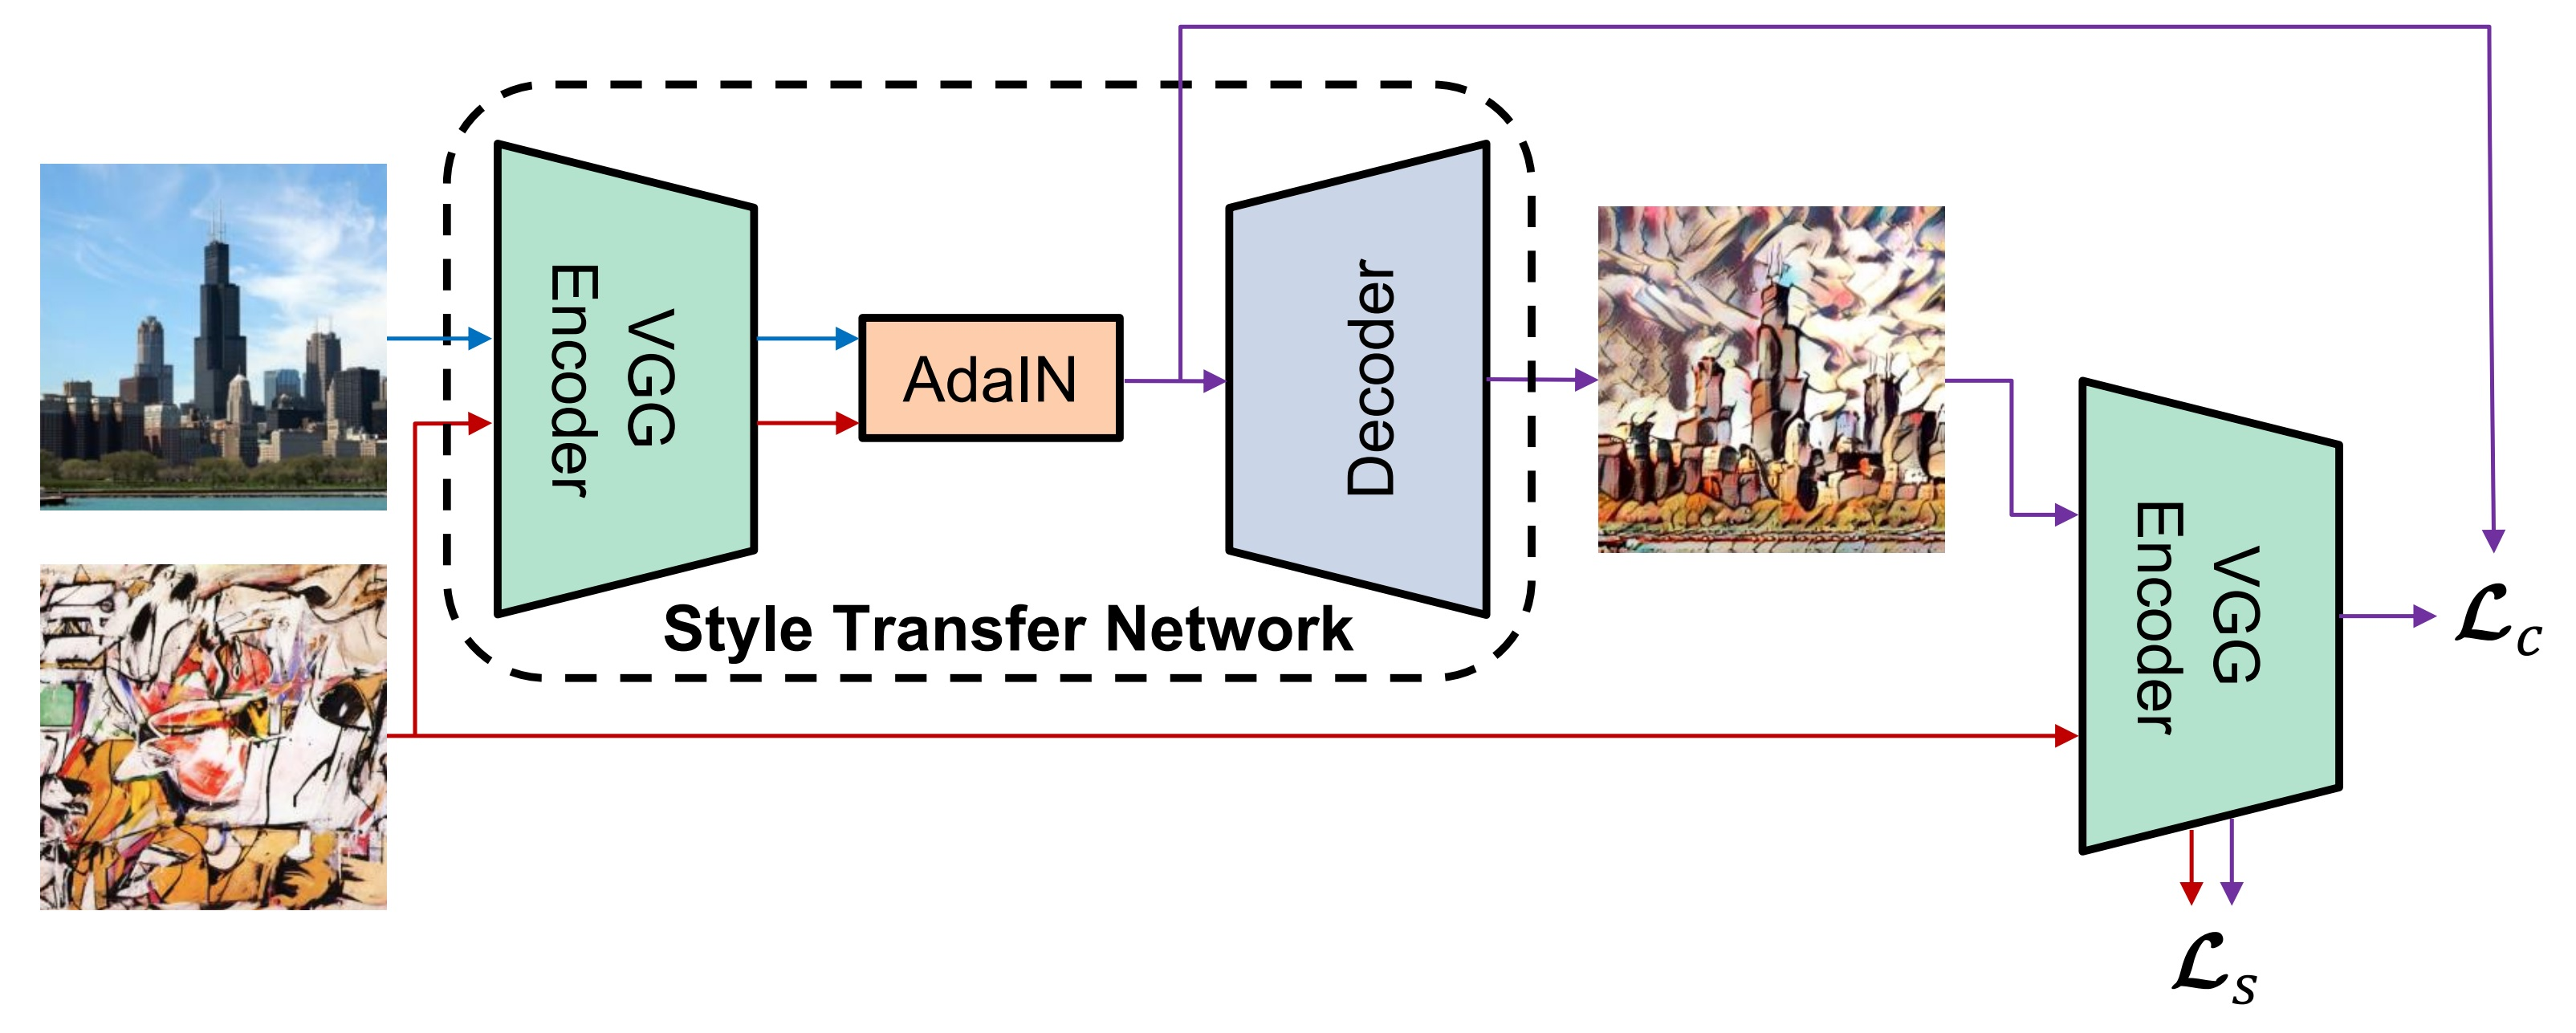
\includegraphics[width=0.45\textwidth]{imgs/adain_architecture}

AdaIN-style is the first real-time style transfer algorithm than can transfer arbitrary new styles.
That means that we can stylize an image with any texture image we want.
This pretrained architecture uses a VGG-19 network to encode the content and style images.
An AdaIN layer is then used to perform style transfer in the feature space.   
A Decoder then decodes the AdaIN output to image space.

\subsection{ResNet}

TODO


\subsection{Cue Conflict ???}

TODO MAYBE ?

\newpage
\section{Experiments}

The authors of the original paper trained multiple models, 
namely Resnet-50, BagNet-33, BagNet-17 and BagNet-9

MODELS
TEXTURES
DATASETS

\subsection{Texture biais hypothesis}
% The first experiment of this analysis was to reproduce the original experiment of the paper with imagenette-160 
% and handpicked images and textures. 
% We then trained a ResNet-18 to classify the chosen images and visualize the results.
% Figure 1 below shows the result of classification for a content image (a), texture image (b) and stylized image (c).

The first experiment conducted by the authors was to validate the texture biais 
through image classification on handpicked stylized subsets. 
Their hypothesis was that the re-texturized image would be classified as the texture representation, rather than 
the underlying content using the shapes, which would be contrary to popular belief. \smallskip

\noindent
We've reproduced their experiment using the picture of an English Springer as our content image (a), 
a colorful parachute as our texture image (b),
and a stylized version of the Springer (c) using AdaIN style transfer 
(Huang \& Belongie, 2017) % TODO: ADD REFERENCE TO STYLE TRANSFER
to introduce a texture-shape cue conflicts. \smallskip

\noindent
The classification results after training the resnet-18 on the imagenette-160 dataset can be seen on figure 1.
We've obtained probabities in line with what was suggested by the authors, 
where the stylized image was recognized as a parachute, 
due to the texture biais, rather than an English Springer.

\begin{figure}[h!]\center
  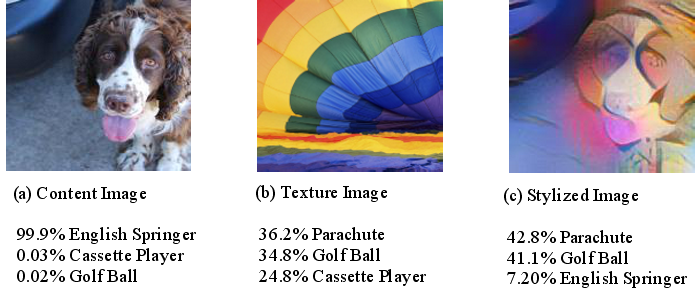
\includegraphics[width=0.47\textwidth]{imgs/results-textures}
  \caption{Classification results after training on imagenette-160.}
\end{figure}

\noindent
Retraining the model on the stylized imagenette-160 dataset with the same parameters 
(resnet-18, 20 epochs, 2e-2 learning rate), led to classification probabities available in figure 2.
As expected, and although the results are a bit less accurate than on the original model, 
we get the correct class prediction for the stylized image, suggesting that our CNN recognized the object
from its shape this time around, having no texture clue to learn from.


\textbf{TODO: FINISH FIGURE 2 AND PUT HERE}

\begin{figure}[h!]\center
  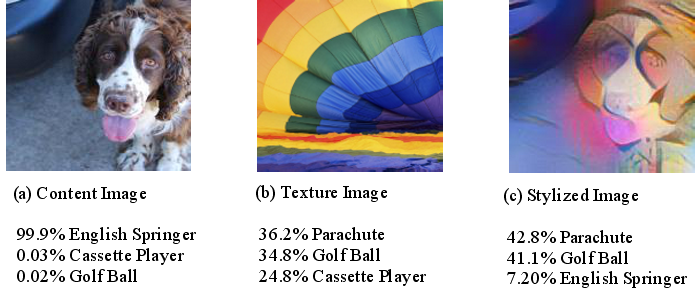
\includegraphics[width=0.47\textwidth]{imgs/results-textures}
  \caption{Classification results with stylized imagenette-160.}
\end{figure}

\subsection{Robustness of shape-based representations}

We reproduce the 4 experiments of the paper to prove the robustness of a shape-biased CNN.
Here, SIN and IN represent Stylized-Imagenette and Imagenette datasets respectively.

\begin{table}[h!]
  \begin{tabular}{lllll}
  \Xhline{2\arrayrulewidth}
  Architecture & IN\_IN & SIN\_SIN & IN\_SIN & SIN\_IN \\ \hline
  ResNet-18    & 0.9    & 0.8      & 0.3     & 0.6     \\ \Xhline{2\arrayrulewidth}
  \end{tabular}
  \caption{Accuracy of ResNet18 model on different tests}
\end{table}


\subsubsection{IN \texorpdfstring{\textrightarrow} .IN}
A model trained on IN and tested on IN is the usual training scheme used in the literature.
It yields competitive results, as we already now.

\begin{figure}[h!]
  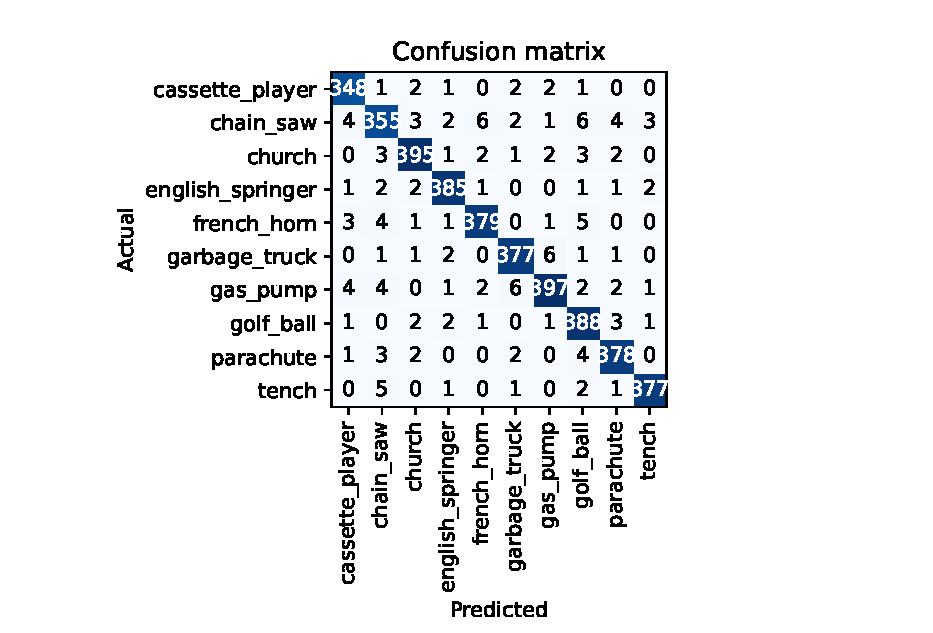
\includegraphics[width = 0.45\textwidth]{imgs/in/in-in/in-in_confusion_matrix_0.963.eps}
  \caption{Confusion Matrix of IN \texorpdfstring{\textrightarrow} .IN}
\end{figure}

\subsubsection{IN \texorpdfstring{\textrightarrow} .SIN}

The original paper trained a model on IN and tested it on SIN which yielded poor results (see Fig.\ref{fig:cm_in-sin}) as 
the model is texture biased, and the SIN dataset is specifically designed to promote shape biased models.

\begin{figure}[h!]
  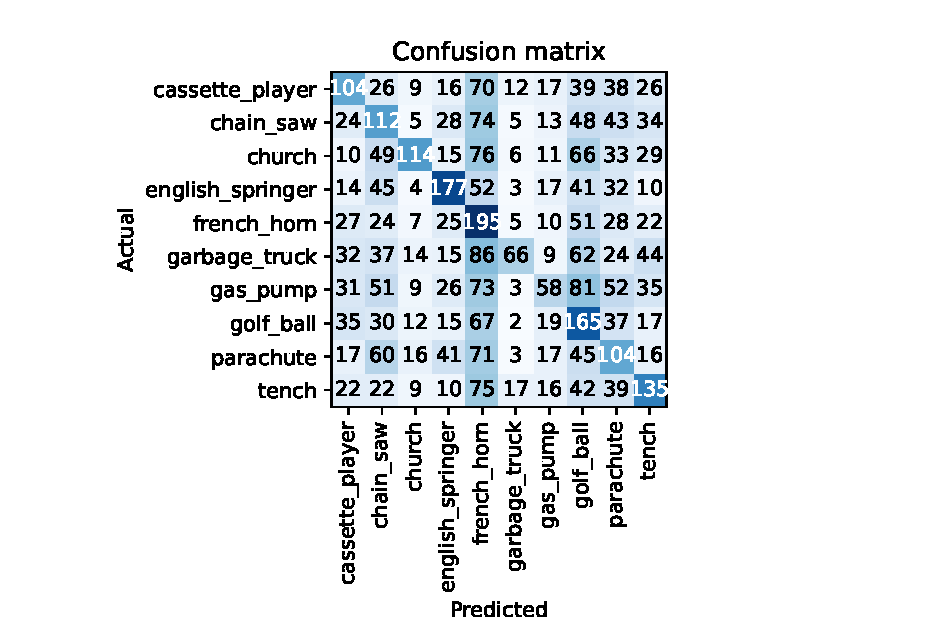
\includegraphics[width = 0.45\textwidth]{imgs/in/in-sin/in-sin_confusion_matrix_0.313.eps}
  \caption{Confusion Matrix of IN \texorpdfstring{\textrightarrow} .IN}
  \label{fig:cm_in-sin}
\end{figure}

\subsubsection{SIN \texorpdfstring{\textrightarrow} .SIN}
This training scheme yields fairly good results. This shows that the model is capable to learn
and generalize on the stylized dataset.

\begin{figure}[h!]
  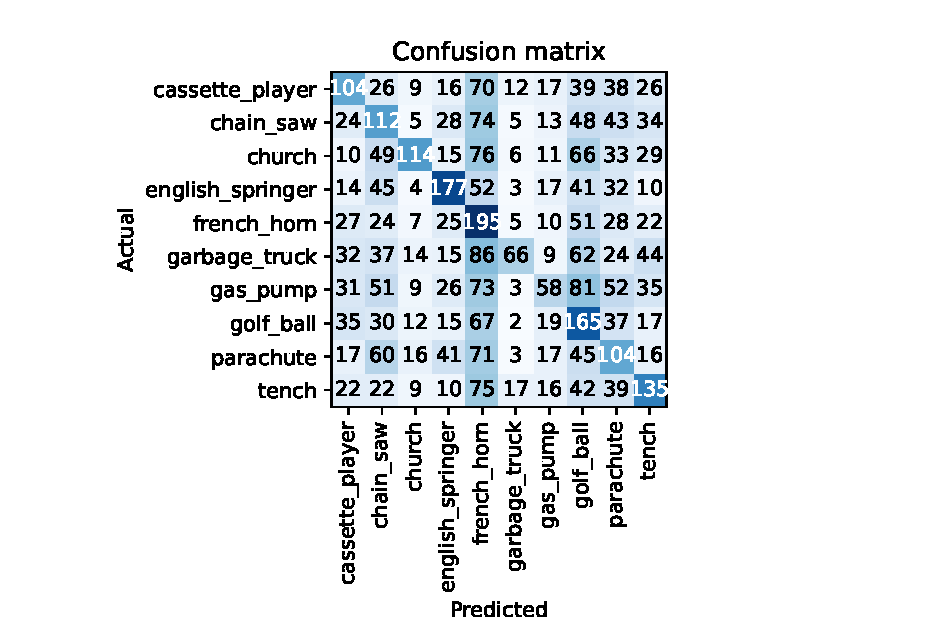
\includegraphics[width = 0.45\textwidth]{imgs/in/in-sin/in-sin_confusion_matrix_0.313.eps}
  \caption{Confusion Matrix of IN \texorpdfstring{\textrightarrow} .IN}
\end{figure}

\subsubsection{SIN \texorpdfstring{\textrightarrow} .IN}

This training scheme yields inferior results than IN \texorpdfstring{\textrightarrow} IIN, however
there are much better than IN \texorpdfstring{\textrightarrow} .SIN.
This demonstrates that a shape-biased model generalizes better than texture biased models.

\subsection{Shape-ResNet}

\subsubsection{SIN + IN \texorpdfstring{\textrightarrow} .IN}

Mixing the 2 datasets has the effect of data augmentation. The model will be better
at generalizing. The results are better than the SIN-only, but worse that IN-only training.
We can interpret these results by the fact IN-only training overfit a lot on texture.

\subsubsection{SIN + IN + finetune(IN) \texorpdfstring{\textrightarrow} .IN}

This method yields the best results, and seem to be the more robust. The finetuning only occurs
on the last layers of the ResNet (the classification layers) and not the feature extracting layers.
Hence, the model does not overfit on textures, but is better to better classify images.

\subsection{Noise resistance}


One of the major finding in the original paper was that the model trained with a shape bias had developed a better resistance to distortions than the regular model.
A model trained to recognize textures should behave differently from one trained to recognize shapes on a noised data set.  The key idea is that not all types of distortions are the same and this model should in theory only be resistant to some of them.  We decided to focus on 3 main types of distortions.  A uniform noise, a high pass filter and a low pass filter.

The result of the original paper show us that the SIN model has a better resistance to uniform noise, high pass filtered image and a worse resistance to low pass filtered images.
This makes sense since a uniform noise has a much worse effect on texture than overall shape. Also, a high pass filter acts as a contour amplifier thus making the shape in the image more prominent. In the same line of thought, a low pass filter has the opposite effect, blurring the edges of an image and making it's shape much less discernible.

\begin{figure}[h!]
\centering
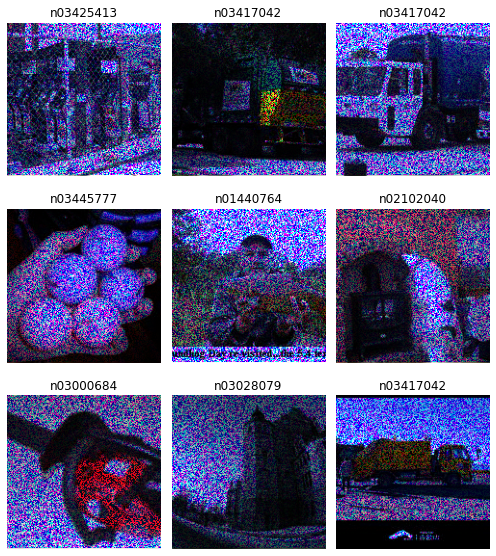
\includegraphics[width = 0.25\textwidth]{imgs/image_uniform}
\caption{uniform noise}
\end{figure}

\begin{figure}[h!]
\centering
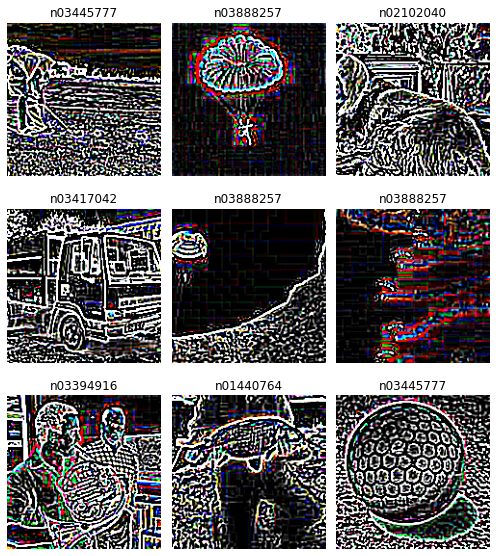
\includegraphics[width = 0.25\textwidth]{imgs/image_high}
\caption{high pass}
\end{figure}

\begin{figure}[h!]
\centering
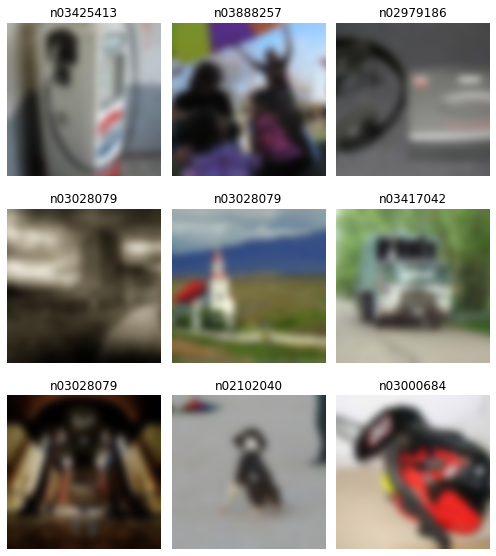
\includegraphics[width = 0.25\textwidth]{imgs/image_low}
\caption{low pass}

\end{figure}

\subsubsection{experiment}

We decided to reproduce this experiment with our own data.
All of the distorted data sets are created form the regular imagenette data set. We applied the distortions at different scale gradually increasing the effect on the images.

We then compared the results of our three trained models against those different noise levels.
The models were the regular resnet trained on imagenette (IN), a resnet trained on a stylised version of imagenette (SIN) and one trained on a combination of this data (SIN+IN).
Each model was given the same test set on which a gradually increasing noise was applied and an accuracy was computed.

The different level of noise were chosen arbitrarily to create different enough distortions. The original values and algorithms used in the paper were not available.

\subsubsection{results}

In all of the test we conducted, the SIN model always start off worse. This is to be expected because it was trained on stylised images and the test set for the distorted images is based on regular images. The IN and SIN+IN model start at about the same accuracy.

\begin{figure}[h!]
\centering
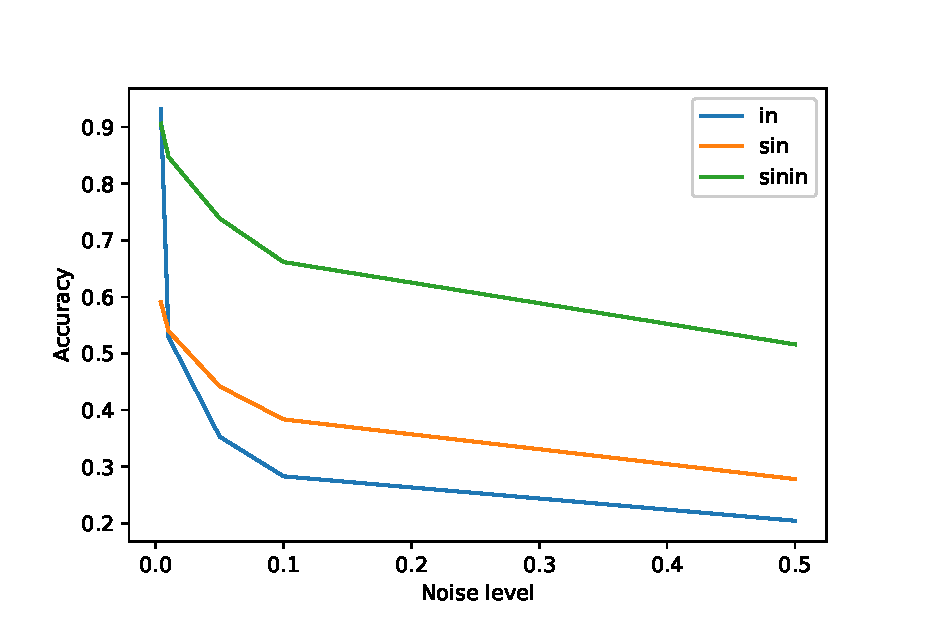
\includegraphics[width = 0.45\textwidth]{imgs/uniform}
\caption{Uniform noise}
\end{figure}

\begin{figure}[h!]
\centering
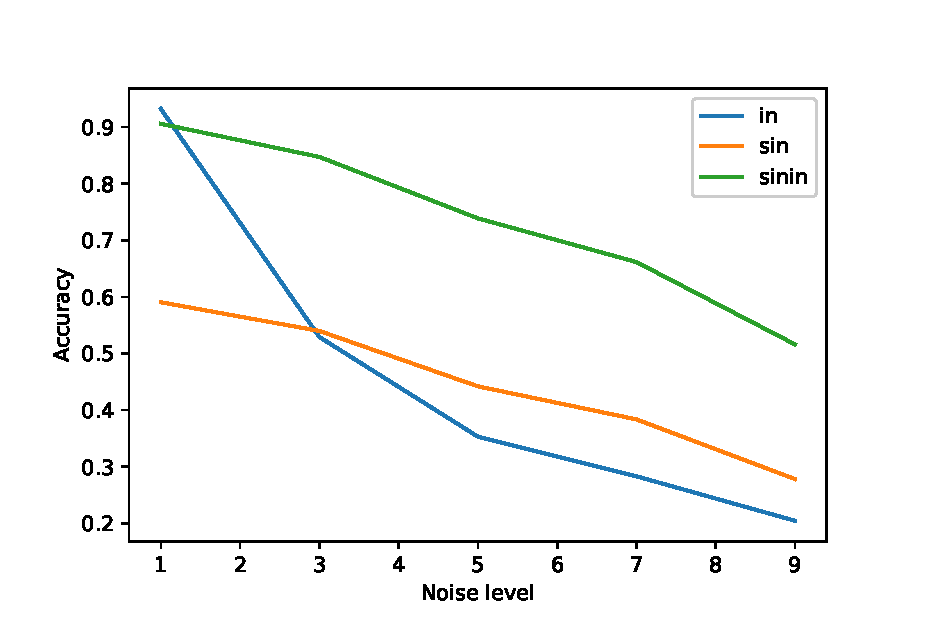
\includegraphics[width = 0.45\textwidth]{imgs/high_pass}
\caption{High noise}
\end{figure}

\begin{figure}[h!]
\centering
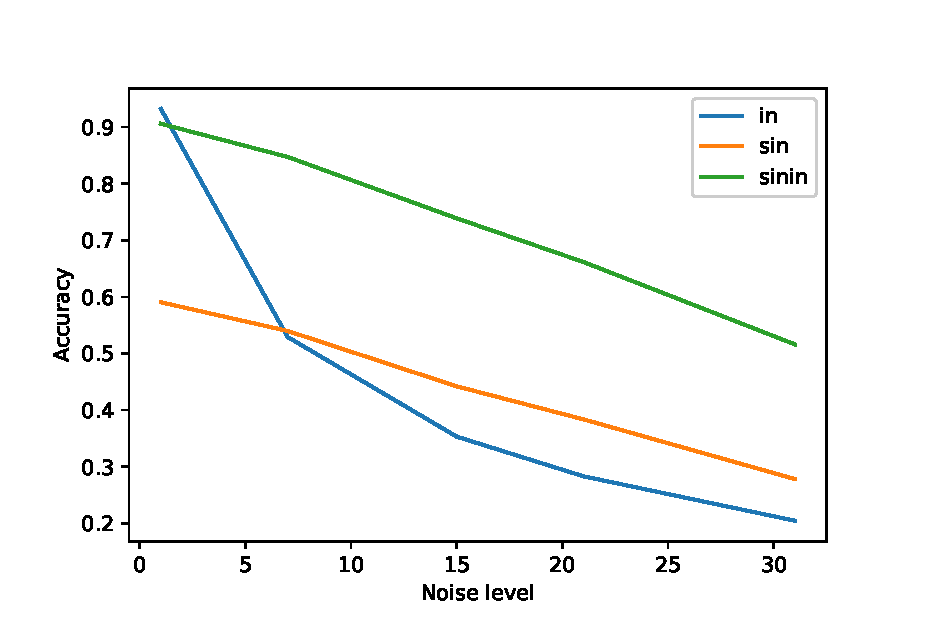
\includegraphics[width = 0.45\textwidth]{imgs/low_pass}
\caption{Low pass}
\end{figure}

The figures clearly show the shape biased models have a better resistance to noise the regular model.

We were surprised by the results for two reasons.
First, the SIN model started off at a worse accuracy, so we were expecting to compare the resistance to distortions as a relative drop from the original accuracy but it managed to have a better absolute accuracy than the regular model.
Secondly, we were expecting the SIN model to under perform in the low pass area, but it managed to be better than the IN model. This goes against the results of the original paper and against common sense. It is possible the levels of blur applied were either too strong or not enough

\section{Approach analysis}

\subsection{Dataset}

We used the same data as the authors: we didn't have time
to find another image classification dataset that fitted our needs.
Many of the datasets we found online were poorly anotated, or the images
were too large.

CIFAR-10's quality was to poor to do style transfer.
%  (include figure in /imgs/dataset_comparison)

The original Imagenet dataset had too many classes and too many images.

It would be interesting to test this approach on a completely different dataset.

\subsection{Results}

Overall, we were able to reproduce their results and
even surpass them. This can be justified by the fact that the classes
in Imagenette were handpicked to be easily classified, and that there were less 
classes than Imagenet.

\subsection{Experiments}

We only reproduced experiments that yielded interesting results 
in the original paper. We can see the excellent quality of the work, 
because their experiments were easily reproducable, and most of the 
steps were clearly explained.

\subsection{Ideas for future studies}

Testing this robustness in related areas were shape bias (like image segmentation) 
is more important than image classification could be interesting.

\section{Conclusion}

This is where we conclude bois hjf

% To begin with, we reproduced the first experiment of the paper. This experiment
% is represents the misconception we have about how CNNs learn.

% Figure Mehdi

% We can see that the pretrained CNN recognized the elephant with just its texture.
% More interestingly, it recognized it classified the cat shape with elephant texture as an elephant.
% The texture hypothesis is more likely to be true.
% Let's define more robust experiments to verify that.

% \newpage
% \subsection{Texture bias of CNNs}

% General explanation

% \subsubsection{IN to IN}
% expected results
% \subsubsection{SIN to IN}
% expected results

% \subsection{Dataset}

% Details on dataset creation

% \subsection{Resistance to noise}

% Experiences Abder
% Data generation

% \subsection{Training}

% Details of ResNet model
% Hyperparams
% Nb Epochs
% FineTuning method

% \section{Results}

% \subsection{Texture bias of CNNs}

% \subsection{Resistance to noise}


% \section{Discussion}

% \subsection{Texture bias of CNNs}

% \subsection{Resistance to noise}

\appendix

%% The file named.bst is a bibliography style file for BibTeX 0.99c
\bibliographystyle{named}
\bibliography{ijcai19}

\end{document}

